\documentclass{article}
\usepackage{xcolor}
\usepackage[a4paper, total={7in, 10in}]{geometry}
\usepackage{enumitem}
\usepackage{listings}
\usepackage{float}
\usepackage{setspace}
\usepackage{textcomp}
\usepackage{amsmath}
\usepackage{mathtools}

\title{\Huge Lista 2}
\author{\Large Arquitetura e Organização de Computadores}
\date{Junho de 2024}

\begin{document}
\large

\maketitle

\begin{enumerate}

\item Traduza o programa abaixo, em C, para MIPS.

\begin{center}
    \begin{minipage}{0.55\textwidth}
        \begin{lstlisting}[frame=single]
int add(int a, int b) {
    int sum;

    sum = a + b;
    return sum;
}

int negative(int a) {
    int neg_a;
    
    neg_a = 0 - a;
    return neg_a;
}

int diff(int a, int b) {
    int neg_b, difference;

    neg_b = negative(b);
    difference = add(a, neg_b);
    return difference;
}

void main() {
    int a, b, c, d;

    c = add(a, b);
    d = diff(a, b);
}
        \end{lstlisting}
    \end{minipage}
\end{center}
\pagebreak
\item Traduza o programa abaixo, em C, para MIPS.

\begin{center}
    \begin{minipage}{0.6\textwidth}
        \begin{lstlisting}[frame=single]
int factorial(int n) {
	if(n == 0) return 1;
	return n * factorial(n - 1);
}

void main()  {
	int num = 5;
        int fact = factorial(num);
}
        \end{lstlisting}
    \end{minipage}
\end{center}

\item Ao fim da execução do programa abaixo, quais os valores em \verb|$sp| e \verb|$s1|? Qual o menor valor armazenado, ao longo da execução deste programa, em \verb|$sp|?

\begin{center}
    \begin{minipage}{0.45\textwidth}
        \begin{lstlisting}[frame=single]
addi $sp, $0, 0x7FFFEFFC
j main

recursive:
lw $t0, 0($sp)
addi $sp, $sp, 4

bne $t0, $0, else
addi $sp, $sp, -4
sw $t0, 0($sp)
jr $ra

else:
addi $t0, $t0, -1
addi $sp, $sp, -8
sw $t0, 0($sp)
sw $ra, 4($sp)
jal recursive
lw $t0, 0($sp)
lw $ra, 4($sp)
addi $sp, $sp, 8
addi $t0, $t0, 1
addi $sp, $sp, -4
sw $t0, 0($sp)
jr $ra

main:
addi $s0, $0, 0xABCD
addi $sp, $sp, -4
sw $s0, 0($sp)
jal recursive
lw $s1, 0($sp)
addi $sp, $sp, 4
        \end{lstlisting}
    \end{minipage}
\end{center}
\pagebreak
\item Ao fim da execução do programa abaixo, como está o banco de registradores?

\begin{center}
    \begin{minipage}{0.45\textwidth}
        \begin{lstlisting}[frame=single]
addi $2, $0, 0xABCD
addi $3, $0, 0xFEDC
multu $2, $3
mflo $4
mfhi $5
mulu $6, $2, $3
mfhi $7

addi $2, $0, 0xABCDEF00
addi $3, $0, 0x00FECDBA
multu $2, $3
mflo $8
mfhi $9
mulu $10, $2, $3
mfhi $11
        \end{lstlisting}
    \end{minipage}
\end{center}
\item Ao fim da execução do programa abaixo, como está o banco de registradores?

\begin{center}
    \begin{minipage}{0.45\textwidth}
        \begin{lstlisting}[frame=single]
addi $2, $0, 0xABCD
addi $3, $0, 0xFEDC
div $2, $3
mflo $4
mfhi $5
divu $2, $3
mflo $6
mfhi $7 

addi $2, $0, 0xABCDEF00
addi $3, $0, 0x00FECDBA
div $2, $3
mflo $8
mfhi $9
divu $2, $3
mflo $10
mfhi $11
        \end{lstlisting}
    \end{minipage}
\end{center}

\item Quais valores hexadecimais podem representar o número \verb|3.462408E-11| conforme a norma IEEE 754?

\item Qual número é armazenado como \verb|0x49179EA0| conforme a norma IEEE 754?

\pagebreak

\item Traduza o programa abaixo, em C, para MIPS.

\begin{center}
    \begin{minipage}{0.475\textwidth}
        \begin{lstlisting}[frame=single]
#include <math.h>

float fop(float a, float b) {
    if(b == 0) return NAN;
    return a*b + a/b;
}

void main() {
    float a = 40.1;
    float b = 00.4;
    float c = fop(a, b);
}
        \end{lstlisting}
    \end{minipage}
\end{center}

Para as questões que pedem a descrição de instruções, considere os processadores apresentados no livro Digital Design and Computer Architecture. Se necessário expandi-lo, indique as alterações feitas.

\item Mostre como as seguintes instruções são executadas em um processador de ciclo único. Para isso, indique quais sinais são transferidos entre quais componentes.

Exemplo: ADD\\

\begin{figure}[H]
    \centering
    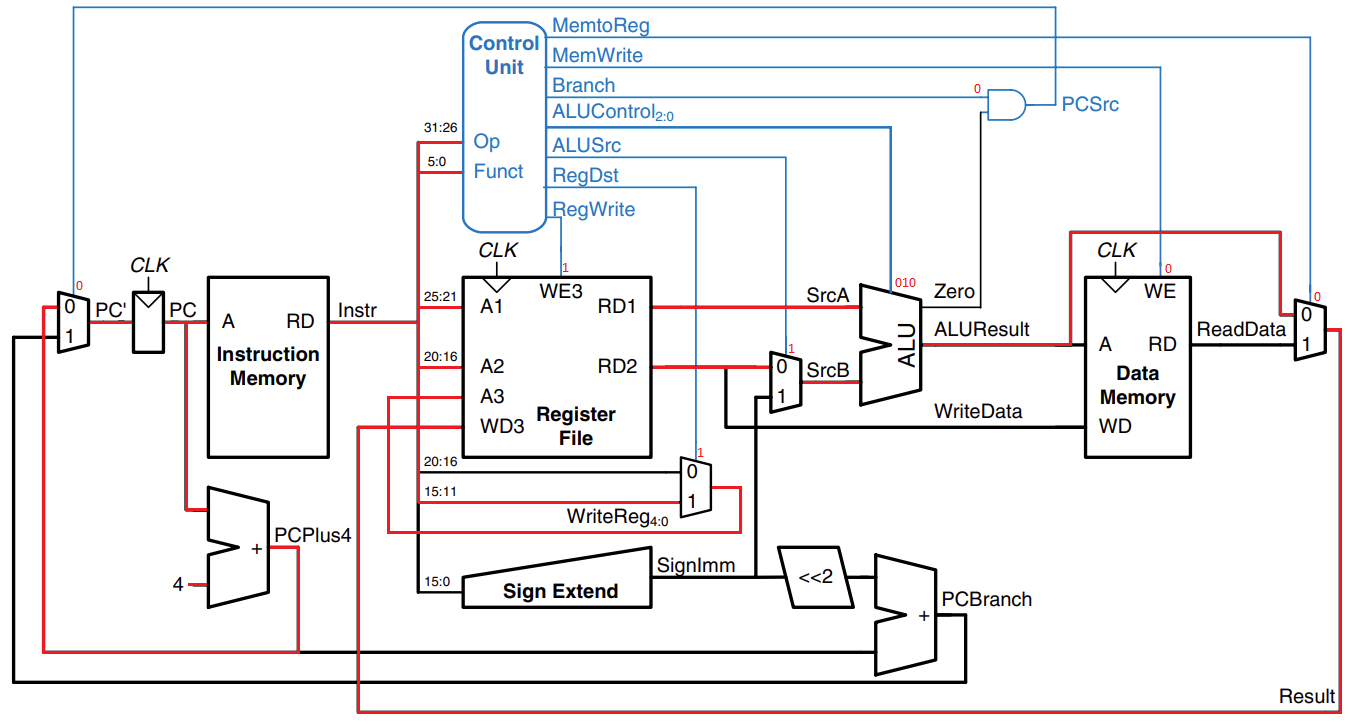
\includegraphics[width=1\linewidth]{add.png}
\end{figure}

\begin{enumerate}
    \item sub
    \item jr
    \item jal
    \item beq
    \item sw
    \item lw
    \item addi
\end{enumerate}

\item Descreva, temporalmente, como as seguintes instruções são executadas em um processador multi-ciclo. Para isso, indique quais sinais são transferidos entre quais componentes.

Exemplo: ADD\\

1 $\text{PC}_\text{reg} \xrightarrow{\text{PC}} \text{Adr}_\text{multiplexer} \xrightarrow{\text{Adr}} \text{Mem} \xrightarrow{\text{Instr/Data}} \text{InstReg}$, $\text{CtrlUnit} \begin{matrix*}[l] 
\xrightarrow{\text{PC}_\text{write}} \text{PCEn}_\text{OR} \xrightarrow{\text{PCEn}} \text{PC}_\text{reg} \\ 
\xrightarrow{\text{PCSrc}} \text{PCSrc}_\text{multiplexer} \\
\xrightarrow{\text{IR}_\text{write}} \text{InstReg} \\
\xrightarrow{\text{IorD}} \text{Adr}_\text{multiplexer} \\ \xrightarrow{\text{ALUSrcA}} \text{SrcA}_\text{multiplexer} \\ \xrightarrow{\text{ALUSrcB}} \text{SrcB}_\text{multiplexer} \\ \xrightarrow{\text{PCSrc}} \text{PCSrc}_\text{multiplexer} \end{matrix*}$,\\ $\begin{matrix*}[r] \text{PC}_\text{reg} \xrightarrow{\text{PC}} \text{SrcA}_\text{multiplexer} \xrightarrow{\text{SrcA}} \\ \text{4} \xrightarrow{\text{4}} \text{SrcB}_\text{multiplexer} \xrightarrow{\text{SrcB}}\end{matrix*} \text{ALU} \xrightarrow{\text{PC+4}} \text{PCSrc}_\text{multiplexer} \xrightarrow{\text{PC+4}} \text{PC}_\text{reg}$\\

\bigbreak

2 $\text{InstReg} \begin{matrix*}[l] 
\xrightarrow{\text{Funct \& Op}} \text{CtrlUnit} \\ \xrightarrow{\text{rt \& rs}} \text{RegFile} \xrightarrow{\text{rd1 \& rd2}} \text{RegFileData}_\text{reg} \\ \end{matrix*}$\\

\bigbreak

3 $\text{RegFileData}_\text{reg} \begin{matrix*}[l] \xrightarrow{\text{A}} \text{SrcA}_\text{multiplexer} \xrightarrow{\text{SrcA}} \\ \xrightarrow{\text{B}} \text{SrcB}_\text{multiplexer} \xrightarrow{\text{SrcB}} \end{matrix*} \text{ALU} \xrightarrow{\text{ALURes}} \text{ALUOut}_\text{reg}$, $\text{CtrlUnit} \begin{matrix*}[l] 
\xrightarrow{\text{ALUCtrl}} \text{ALU} \\ \xrightarrow{\text{ALUSrcA}} \text{SrcA}_\text{multiplexer} \\ \xrightarrow{\text{ALUSrcB}} \text{SrcB}_\text{multiplexer} \end{matrix*}$\\

\bigbreak

4 $\text{ALUOut}_\text{reg} \xrightarrow{\text{ALUOut}} \text{WD3}_\text{multiplexer} \xrightarrow{\text{ALUOut}} \text{WD3}_\text{RegFile}$,  $\text{CtrlUnit} \begin{matrix*}[l] 
\xrightarrow{\text{RegDst}} \text{RegDst}_\text{multiplexer} \\ \xrightarrow{\text{MemtoReg}} \text{WD3}_\text{multiplexer} \\ \xrightarrow{\text{RegWrite}} \text{RegFile} \end{matrix*}$\\


\begin{enumerate}
    \item sub
    \item jr
    \item jal
    \item beq
    \item sw
    \item lw
    \item addi
\end{enumerate}

Para as 8 seguintes questões, considere um processador pipeline que implemente todas as tratativas de hazards.

\item Em qual estágio o registrador de \verb|PC| é incrementado? Em qual estágio o novo valor é disponibilizado à memória de instruções? Em quais condições o valor anterior é mantido para a próxima execução?

\item Em qual estágio a tratativa de data hazards para \verb|lw| é feita? Qual condição é verificada nesta tratativa? Quando este tipo de hazard é detectado, como é tratado?

\item Descreva como, no estágio \textbf{Execute}, é feita a avaliação e tratativa de hazards.

\item Quais sinais, no estágio \textbf{Memory}, contribuem para a detecção ou tratativa de hazards? Como estes são avaliados ou utilizados?

\item Quais sinais, no estágio \textbf{WriteBack}, contribuem para a detecção ou tratativa de hazards? Como estes são avaliados ou utilizados?

\item Em qual estágio de uma instrução \verb|beq| os hazards pertinentes a ela são detectados? Como estes são avaliados e tratados?

\item Em um processador pipeline, o que significar, "limpar" ou "resetar" um registrador de pipeline? Como isso impede a continuação da instrução a partir do estágio em que ocorre?

\item No processador pipeline implementado no livro de referência, é possível realizar forwarding do estágio \textbf{WriteBack} para o estágio \textbf{Memory}? Em qual condição isto é necessário? Qual a justificativa para a decisão tomada na implementação apresentada pelo livro?

Para as próximas duas questões, considere o programa abaixo.

\begin{center}
    \begin{minipage}{0.35\textwidth}
        \begin{lstlisting}[frame=single]
i00: addi $s0, $0, 10
i01: sw   $s0, 0($sp)
i02: addi $s0, $0, 2
i03: addi $s1, $0, 3
i04: add  $s2, $s1, $s0
i05: sub  $s1, $s2, $s0
i06: lw   $s3, 0($sp)
i07: add  $s4, $s3, $s3
i08: beq  $s4, $s3, one
i09: add  $s0, $0, $0
i10: add  $s1, $0, $0
i11: add  $s2, $0, $0
i12: add  $s3, $0, $0
i13: beq  $0, $0, zero
one:
i14: add  $s0, $0, 1
i15: add  $s1, $0, 1
i16: add  $s2, $0, 1
i17: add  $s3, $0, 1
zero:
i18: add  $s6, $s2, $s3
i19: add  $s5, $s0, $s1
i20: add  $s7, $s6, $s5
        \end{lstlisting}
    \end{minipage}
\end{center}

\pagebreak

\item Considerando uma arquitetura que detecte hazards, mas não empregue forwarding, indique, na tabela abaixo, em qual estágio cada instrução está em cada ciclo de clock. Utilize as células da coluna reservada para indicar a instrução executada. Reserve, conforme necessário, linhas para indicar os ciclos de clock.

\begin{table}[H]
\begin{tabular}{|l|l|l|l|l|l|l|l|l|l|l|l|l|l|l|l|l|l|}
\hline
inst\textbackslash ciclo & C0  & C1  & C2  & C3  & C4  & C5  & C6  & C7  & C8  & C9  & C10 & C11 & C12 & C13 & C14 & C15 & C16 \\ \hline
i0:  &     &     &     &     &     &     &     &     &     &     &     &     &     &     &     &     &     \\ \hline
i1:  &     &     &     &     &     &     &     &     &     &     &     &     &     &     &     &     &     \\ \hline
  &     &     &     &     &     &     &     &     &     &     &     &     &     &     &     &     &     \\ \hline
  &     &     &     &     &     &     &     &     &     &     &     &     &     &     &     &     &     \\ \hline
  &     &     &     &     &     &     &     &     &     &     &     &     &     &     &     &     &     \\ \hline
  &     &     &     &     &     &     &     &     &     &     &     &     &     &     &     &     &     \\ \hline
  &     &     &     &     &     &     &     &     &     &     &     &     &     &     &     &     &     \\ \hline
  &     &     &     &     &     &     &     &     &     &     &     &     &     &     &     &     &     \\ \hline
  &     &     &     &     &     &     &     &     &     &     &     &     &     &     &     &     &     \\ \hline
  &     &     &     &     &     &     &     &     &     &     &     &     &     &     &     &     &     \\ \hline
 &     &     &     &     &     &     &     &     &     &     &     &     &     &     &     &     &     \\ \hline
 &     &     &     &     &     &     &     &     &     &     &     &     &     &     &     &     &     \\ \hline
 &     &     &     &     &     &     &     &     &     &     &     &     &     &     &     &     &     \\ \hline
 &     &     &     &     &     &     &     &     &     &     &     &     &     &     &     &     &     \\ \hline
 &     &     &     &     &     &     &     &     &     &     &     &     &     &     &     &     &     \\ \hline
 &     &     &     &     &     &     &     &     &     &     &     &     &     &     &     &     &     \\ \hline
 &     &     &     &     &     &     &     &     &     &     &     &     &     &     &     &     &     \\ \hline
 &     &     &     &     &     &     &     &     &     &     &     &     &     &     &     &     &     \\ \hline
 &     &     &     &     &     &     &     &     &     &     &     &     &     &     &     &     &     \\ \hline
 &     &     &     &     &     &     &     &     &     &     &     &     &     &     &     &     &     \\ \hline
 &     &     &     &     &     &     &     &     &     &     &     &     &     &     &     &     &     \\ \hline
 &     &     &     &     &     &     &     &     &     &     &     &     &     &     &     &     &     \\ \hline
 &     &     &     &     &     &     &     &     &     &     &     &     &     &     &     &     &     \\ \hline
  &     &     &     &     &     &     &     &     &     &     &     &     &     &     &     &     &     \\ \hline
  &     &     &     &     &     &     &     &     &     &     &     &     &     &     &     &     &     \\ \hline
  &     &     &     &     &     &     &     &     &     &     &     &     &     &     &     &     &     \\ \hline
  &     &     &     &     &     &     &     &     &     &     &     &     &     &     &     &     &     \\ \hline
  &     &     &     &     &     &     &     &     &     &     &     &     &     &     &     &     &     \\ \hline
  &     &     &     &     &     &     &     &     &     &     &     &     &     &     &     &     &     \\ \hline
  &     &     &     &     &     &     &     &     &     &     &     &     &     &     &     &     &     \\ \hline
  &     &     &     &     &     &     &     &     &     &     &     &     &     &     &     &     &     \\ \hline
  &     &     &     &     &     &     &     &     &     &     &     &     &     &     &     &     &     \\ \hline
  &     &     &     &     &     &     &     &     &     &     &     &     &     &     &     &     &     \\ \hline
 &     &     &     &     &     &     &     &     &     &     &     &     &     &     &     &     &     \\ \hline
 &     &     &     &     &     &     &     &     &     &     &     &     &     &     &     &     &     \\ \hline
 &     &     &     &     &     &     &     &     &     &     &     &     &     &     &     &     &     \\ \hline
 &     &     &     &     &     &     &     &     &     &     &     &     &     &     &     &     &     \\ \hline
 &     &     &     &     &     &     &     &     &     &     &     &     &     &     &     &     &     \\ \hline
 &     &     &     &     &     &     &     &     &     &     &     &     &     &     &     &     &     \\ \hline
 &     &     &     &     &     &     &     &     &     &     &     &     &     &     &     &     &     \\ \hline
 &     &     &     &     &     &     &     &     &     &     &     &     &     &     &     &     &     \\ \hline
 &     &     &     &     &     &     &     &     &     &     &     &     &     &     &     &     &     \\ \hline
 &     &     &     &     &     &     &     &     &     &     &     &     &     &     &     &     &     \\ \hline
 &     &     &     &     &     &     &     &     &     &     &     &     &     &     &     &     &     \\ \hline
 &     &     &     &     &     &     &     &     &     &     &     &     &     &     &     &     &     \\ \hline
 &     &     &     &     &     &     &     &     &     &     &     &     &     &     &     &     &     \\ \hline
\end{tabular}
\end{table}

\pagebreak

\item Considerando uma arquitetura que detecte hazards e empregue forwarding, stall e previsão de desvio (assume que não é tomado) indique, na tabela abaixo, em qual estágio cada instrução está em cada ciclo de clock. Neste exercício, não se restrinja ao processador implementado no livro. Indique os recursos que achar pertinentes. Utilize as células da coluna reservada para indicar a instrução executada. Reserve, conforme necessário, linhas para indicar os ciclos de clock.

\begin{table}[H]
\begin{tabular}{|l|l|l|l|l|l|l|l|l|l|l|l|l|l|l|l|l|l|}
\hline
inst\textbackslash ciclo & C0  & C1  & C2  & C3  & C4  & C5  & C6  & C7  & C8  & C9  & C10 & C11 & C12 & C13 & C14 & C15 & C16 \\ \hline
i0:  &     &     &     &     &     &     &     &     &     &     &     &     &     &     &     &     &     \\ \hline
i1:  &     &     &     &     &     &     &     &     &     &     &     &     &     &     &     &     &     \\ \hline
  &     &     &     &     &     &     &     &     &     &     &     &     &     &     &     &     &     \\ \hline
  &     &     &     &     &     &     &     &     &     &     &     &     &     &     &     &     &     \\ \hline
  &     &     &     &     &     &     &     &     &     &     &     &     &     &     &     &     &     \\ \hline
  &     &     &     &     &     &     &     &     &     &     &     &     &     &     &     &     &     \\ \hline
  &     &     &     &     &     &     &     &     &     &     &     &     &     &     &     &     &     \\ \hline
  &     &     &     &     &     &     &     &     &     &     &     &     &     &     &     &     &     \\ \hline
  &     &     &     &     &     &     &     &     &     &     &     &     &     &     &     &     &     \\ \hline
  &     &     &     &     &     &     &     &     &     &     &     &     &     &     &     &     &     \\ \hline
 &     &     &     &     &     &     &     &     &     &     &     &     &     &     &     &     &     \\ \hline
 &     &     &     &     &     &     &     &     &     &     &     &     &     &     &     &     &     \\ \hline
 &     &     &     &     &     &     &     &     &     &     &     &     &     &     &     &     &     \\ \hline
 &     &     &     &     &     &     &     &     &     &     &     &     &     &     &     &     &     \\ \hline
 &     &     &     &     &     &     &     &     &     &     &     &     &     &     &     &     &     \\ \hline
 &     &     &     &     &     &     &     &     &     &     &     &     &     &     &     &     &     \\ \hline
 &     &     &     &     &     &     &     &     &     &     &     &     &     &     &     &     &     \\ \hline
 &     &     &     &     &     &     &     &     &     &     &     &     &     &     &     &     &     \\ \hline
 &     &     &     &     &     &     &     &     &     &     &     &     &     &     &     &     &     \\ \hline
 &     &     &     &     &     &     &     &     &     &     &     &     &     &     &     &     &     \\ \hline
 &     &     &     &     &     &     &     &     &     &     &     &     &     &     &     &     &     \\ \hline
 &     &     &     &     &     &     &     &     &     &     &     &     &     &     &     &     &     \\ \hline
 &     &     &     &     &     &     &     &     &     &     &     &     &     &     &     &     &     \\ \hline
  &     &     &     &     &     &     &     &     &     &     &     &     &     &     &     &     &     \\ \hline
  &     &     &     &     &     &     &     &     &     &     &     &     &     &     &     &     &     \\ \hline
  &     &     &     &     &     &     &     &     &     &     &     &     &     &     &     &     &     \\ \hline
  &     &     &     &     &     &     &     &     &     &     &     &     &     &     &     &     &     \\ \hline
  &     &     &     &     &     &     &     &     &     &     &     &     &     &     &     &     &     \\ \hline
  &     &     &     &     &     &     &     &     &     &     &     &     &     &     &     &     &     \\ \hline
  &     &     &     &     &     &     &     &     &     &     &     &     &     &     &     &     &     \\ \hline
  &     &     &     &     &     &     &     &     &     &     &     &     &     &     &     &     &     \\ \hline
  &     &     &     &     &     &     &     &     &     &     &     &     &     &     &     &     &     \\ \hline
  &     &     &     &     &     &     &     &     &     &     &     &     &     &     &     &     &     \\ \hline
 &     &     &     &     &     &     &     &     &     &     &     &     &     &     &     &     &     \\ \hline
 &     &     &     &     &     &     &     &     &     &     &     &     &     &     &     &     &     \\ \hline
 &     &     &     &     &     &     &     &     &     &     &     &     &     &     &     &     &     \\ \hline
 &     &     &     &     &     &     &     &     &     &     &     &     &     &     &     &     &     \\ \hline
 &     &     &     &     &     &     &     &     &     &     &     &     &     &     &     &     &     \\ \hline
 &     &     &     &     &     &     &     &     &     &     &     &     &     &     &     &     &     \\ \hline
 &     &     &     &     &     &     &     &     &     &     &     &     &     &     &     &     &     \\ \hline
 &     &     &     &     &     &     &     &     &     &     &     &     &     &     &     &     &     \\ \hline
 &     &     &     &     &     &     &     &     &     &     &     &     &     &     &     &     &     \\ \hline
 &     &     &     &     &     &     &     &     &     &     &     &     &     &     &     &     &     \\ \hline
 &     &     &     &     &     &     &     &     &     &     &     &     &     &     &     &     &     \\ \hline
 &     &     &     &     &     &     &     &     &     &     &     &     &     &     &     &     &     \\ \hline
 &     &     &     &     &     &     &     &     &     &     &     &     &     &     &     &     &     \\ \hline
\end{tabular}
\end{table}

\pagebreak

\item Reorganize o programa a seguir a fim de evitar hazards sem alterar seu estado final.

\begin{center}
    \begin{minipage}{0.3\textwidth}
        \begin{lstlisting}[frame=single]
or   $t2, $t1, $t0
nor  $t9, $t8, $t7
addi $s2, $s1, 1
add  $s2, $s1, $s0
sub  $s4, $s3, $s2
xor  $t2, $t1, $t0
sw   $t2, 0($sp)
lw   $t9, 4($sp)
subi $t0, $t0, 1
and  $t7, $t8, $t9
        \end{lstlisting}
    \end{minipage}
\end{center}



\end{enumerate}
\end{document}
